\subsection{Consistent replacement and comparison conditions}
The three resolved H$\alpha$ branches now use a common static,
complete-redistribution transfer solution in spherical shells. Their upward
and downward rates replace the native escape/shielding rates, and their
old on-the-spot source events are removed. Local self-emission is eliminated
analytically in the population operator. A continuation weight applies to
all these replacements together; the physical endpoint has weight one.

Within the finite H$\alpha$ window, the continuum-receiver correction is
\begin{equation}
 \Delta\Phi_\nu=\frac{4\pi w_\nu}{h\nu}
 \left(J_\nu^{\mathrm{sphere,line+continuum}}
       -J_\nu^{\mathrm{represented\ background}}\right).
\end{equation}
The reference is the actual global continuum field used by the native
rates. Subtracting a separate spherical continuum solution instead would
leave inconsistent background fields in the line and continuum receivers.
The signed correction goes to all retained absorbing species and the
free-free heat ledger, together with the line redistribution heat.
The full stellar spectrum is sampled at the new line-transfer nodes.
Existing H/O overlap and resolved infrared groups remain coupled.
The recorded background-replacement term includes geometry, exact stellar
line sampling versus reconstruction of the global continuum bins, and
finite-quadrature differences. Despite its internal diagnostic name, it is
not an isolated geometry term. Increasing the window changes the extent of
this replacement as well as retaining more line wings; the numerical
controls therefore report the line and background contributions separately.

The comparison fixes the mass loss at
$1.051271096376025\times10^{13}$ g\,s$^{-1}$, the original eight shell edges,
the atom, composition, boundary spectrum, and prescribed lower two LTE
cells. Temperature, populations, electron density and the resulting wind
are re-evaluated. Static line transfer remains an approximation; this solve
does not incorporate the moving-ray diagnostic into the population rates.
It therefore tests the replacement of the original H$\alpha$ closure by
resolved spherical transfer, rather than an isolated spherical-minus-slab
effect with both closures already resolved.

The native observation comparison uses the same nights, orders, pixel
selection, phase integration, stellar division, and fixed GP covariance.
Both spectra are compared with the same bounds for common radial velocity
and amplitude, with a second comparison holding these nuisance parameters
at the baseline optimum. An alternate pixel selection tests sensitivity to
the sampling. We report $\Delta Q=Q_{\rm baseline}-Q_{\rm new}$, so positive
values mean a smaller GP-weighted residual. Displayed residuals are
common-reference log-flux residuals expressed in ppm: data minus the
combined planet and conditional GP prediction, not the predicted
planet-plus-GP profile itself.

\subsection{Complete equilibrium and independent CPU evaluation}
The accelerated solve reached a complete residual of
$1.45845\times10^{-10}$ in maximum norm, with zero change on a fresh
evaluation. An independent CPU evaluation at exactly the same coordinates
gave $1.45856\times10^{-10}$; the maximum CPU--GPU residual difference was
$1.46\times10^{-13}$. Every physical and wind guard passed, and the largest
nuclei, charge or pressure conservation error was $4.44\times10^{-16}$.
No coordinate adjustment was used in this independent comparison.
These are equilibrium checks, not measures of agreement with the data.

\subsection{Observed residuals}
The observed fit worsens. On the primary pixel selection,
$\Delta Q=-65.98282$ after profiling the same two nuisance parameters.
Holding them at the original optimum gives $\Delta Q=-74.55602$.
The complementary pixels give $\Delta Q=-59.81179$ after profiling.
Each of the four night/order contributions also worsens on the primary
selection. The blue residual increases from $+409.06$ to $+594.61$ ppm,
and the central residual from $-235.24$ to $-529.90$ ppm: both discrepancies
grow in magnitude (Table~\ref{tab:halpha-fit} and
Figure~\ref{fig:halpha-observed}).

\begin{table}[htbp]
\centering
\small
\setlength{\tabcolsep}{3pt}
\caption{Identical native observation processing and fixed GP covariance.
RV is in km\,s$^{-1}$; blue and core entries are data-minus-total-prediction
log-flux residuals in ppm. The total prediction includes the conditional GP.}
\label{tab:halpha-fit}
\begin{tabular}{llrrrrr}
\toprule
Pixels & Template and nuisance treatment & $Q$ & RV & $A$ & Blue & Core\\
\midrule
Primary & Baseline; profiled & 38326.65 & 2.8602 & 1.1321 & $+409.06$ & $-235.24$\\
Primary & Coupled; baseline RV/$A$ & 38401.20 & 2.8602 & 1.1321 & $+549.03$ & $-560.50$\\
Primary & Coupled; profiled & 38392.63 & 5.2001 & 1.0489 & $+594.61$ & $-529.90$\\
Alternate & Baseline; profiled & 38012.94 & 3.8283 & 1.0867 & $+309.60$ & $-206.82$\\
Alternate & Coupled; baseline RV/$A$ & 38079.60 & 3.8283 & 1.0867 & $+444.10$ & $-508.42$\\
Alternate & Coupled; profiled & 38072.75 & 5.6008 & 1.0135 & $+476.61$ & $-488.04$\\
\bottomrule
\end{tabular}
\end{table}

The refined observer changes the primary and complementary scores by
$-0.1154$ and $+0.0319$, respectively, relative to the coarser rendering.
At fixed nuisance parameters, every native prediction changes by less than
0.0019 of its white-noise standard deviation. The observed worsening is
therefore stable to this rendering refinement. White-error band averaging
and plotted error bars do not provide a GP-correlated significance test.
Five additional velocity starts spanning $-15$ to $+15$ km\,s$^{-1}$
converge to the same alignment for both templates and pixel selections;
their best scores differ from the reported values by less than
$8\times10^{-10}$. This checks the tested starts rather than proving a
global optimum.

For reference, re-evaluating the saved free-model~\#1 spectra with the same
observation operator and covariance reproduces $Q=38304.82193$ for the
original fixed shape and $Q=38288.89491$ for the previously optimized shape.
No new \#1 fit was performed. The latter has additional shape freedom and
is a descriptive reference, not an equal-complexity evidence comparison.

\begin{figure}[htbp]
\centering
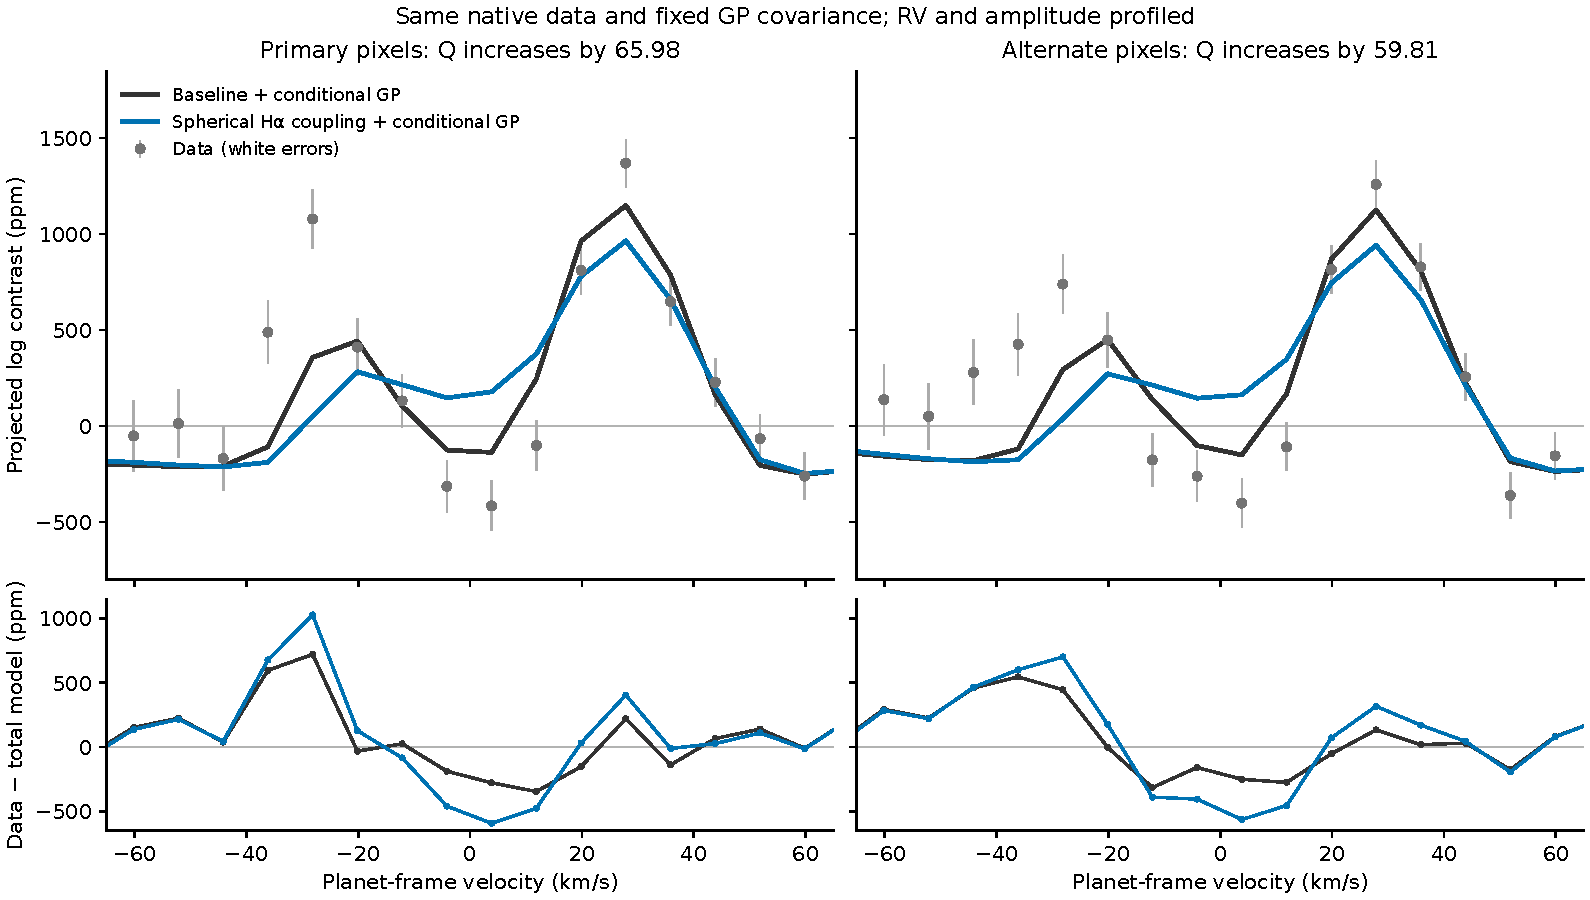
\includegraphics[width=\linewidth]{../mceg/evidence/halpha_geometry_fit_20261126/observed_comparison.pdf}
\caption{Observed projected profiles (top) and data-minus-total-prediction
residuals (bottom), using the finer renderer and separately profiled RV and
amplitude. Both pixel selections show a weaker blue peak and a shallower
central depression with the new coupling. Error bars use the white-error
projection; the fit score uses the unchanged full GP covariance.}
\label{fig:halpha-observed}
\end{figure}

\subsection{Physical response}
The re-solved populations move away from the source-function contrast needed
to brighten the blue peak while deepening the central depression.
Table~\ref{tab:halpha-response} compares the inner emitting shell and the
principal upper receiving shell identified by the earlier transfer diagnosis.
The inner branch source functions decrease by about 15.5\%, while the upper
ones increase by 44--48\%. Consequently the inner/upper source-function ratio
falls to 0.569--0.585 of its original value. The temperature and opacity
changes in these shells are much smaller. This response includes the full
population and thermal feedback; it is not an imposed source-function scale.

\begin{table}[ht]
\centering
\caption{Changes relative to the original equilibrium. Source-function ranges
cover the three H$\alpha$ branches. Optical depth is the total radial line
optical depth at the branch centers, excluding continuum and intercell
Doppler shifts; the observed spectrum retains the actual velocities.}
\label{tab:halpha-response}
\begin{tabular}{lrr}
\toprule
Quantity & Inner ($1.2583R_p$) & Upper ($1.5125R_p$)\\
\midrule
Temperature & $+0.146\%$ & $-0.060\%$\\
$n_2$ & $+3.98\%$ & $-2.41\%$\\
$n_3$ & $-11.91\%$ & $+43.12\%$\\
$S_{\rm branch}$ & $-15.5\%$ & $+44.4$ to $+48.4\%$\\
Radial line optical depth & $+4.21\%$ & $-2.59\%$\\
\bottomrule
\end{tabular}
\end{table}

\subsection{Transfer-resolution controls at the accepted state}
Doubling the angular order from 32 to 64 and the frequency order from 8 to
16 changes the effective upward/downward coefficients by less than
$8\times10^{-8}$ relatively. These coefficients eliminate local
self-emission analytically; they are not gross absorption and emission
rates. All checked transfer solutions remain valid and satisfy the finite
photon and line-energy identities to rounding precision.

Increasing the wing extent from 30 to 60 Doppler widths changes these
effective coefficients by at most $1.58\times10^{-4}$ relatively.
The net H$\alpha$ excitation changes by 0.0845\% in the principal upper shell
and by at most 0.930\% among the non-LTE shells. Larger relative changes in
a small net balance reflect cancellation. The background-replacement
receiving heat grows with the wider window. The change in the H/free-free/
redistribution heat subtotal remains below $1.3\times10^{-5}$ of the
corresponding thermal scale; metal receivers are not included in this
subtotal. These checks separate line and background terms. They do not constitute a
new equilibrium at each refined quadrature, or an uncertainty bound on the
observed score.

\subsection{Audit of the earlier conditional recycling calculation}
The earlier saved radiation-rate object omitted receiving photoionization
and recombination terms added later in the complete population equations.
Restoring those terms in the reduced conditional network changes the primary
outer H$\alpha$ probability from $0.790087363$ to $0.790025288$.
The Ly$\beta$ branch-deletion difference changes from $0.000533967$ to
$0.000533619$. This small correction does not change the earlier mechanism
ranking. The original receipts remain historical records; the correction
is recorded separately. The coupled solver exports the complete hydrogen
rates, including receiving terms, for subsequent audits.
